\section*{Введение}\label{section:secIntro}

В настоящее время на строящемся ускорительном комплексе FAIR (Facility for Antiproton and Ion Research, Дармштадт, Германия)~\cite{FAIR} ведутся работы по созданию экспериментальной установки CBM (Compressed Baryonic Matter)~\cite{CBMBook, CBMSIS100, CBM_TSR, ProgressReport2014}. Физическая программа CBM нацелена на всестороннее изучение фазовой диаграммы сильновзаимодействующей материи и уравнения состояния вещества при экстремально высоких плотностях барионной материи, получаемых при столкновении релятивистских ядер в эксперименте с фиксированной мишенью.

Для реализации программы необходимы измерения выходов и распределений в фазовом пространстве частиц, рождающихся в области взаимодействия. Для этого в каждом событии требуются:
\begin{itemize}
\item {восстановление короткоживущих частиц, включая очень редкие, по продуктам их распадов;}
\item {идентификация долгоживущих продуктов взаимодействия;}
\item {измерение центральности соударения;}
\item {определение плоскости реакции.}
\end{itemize}

Для выполнения различных измерений CBM будет функционировать в двух конфигурациях --- с мюонным детектором (MUCH) и с детектором черенковских колец (RICH).

Схема экспериментальной установки с RICH представлена на \figref{fig:CBM}.

\begin{figure}
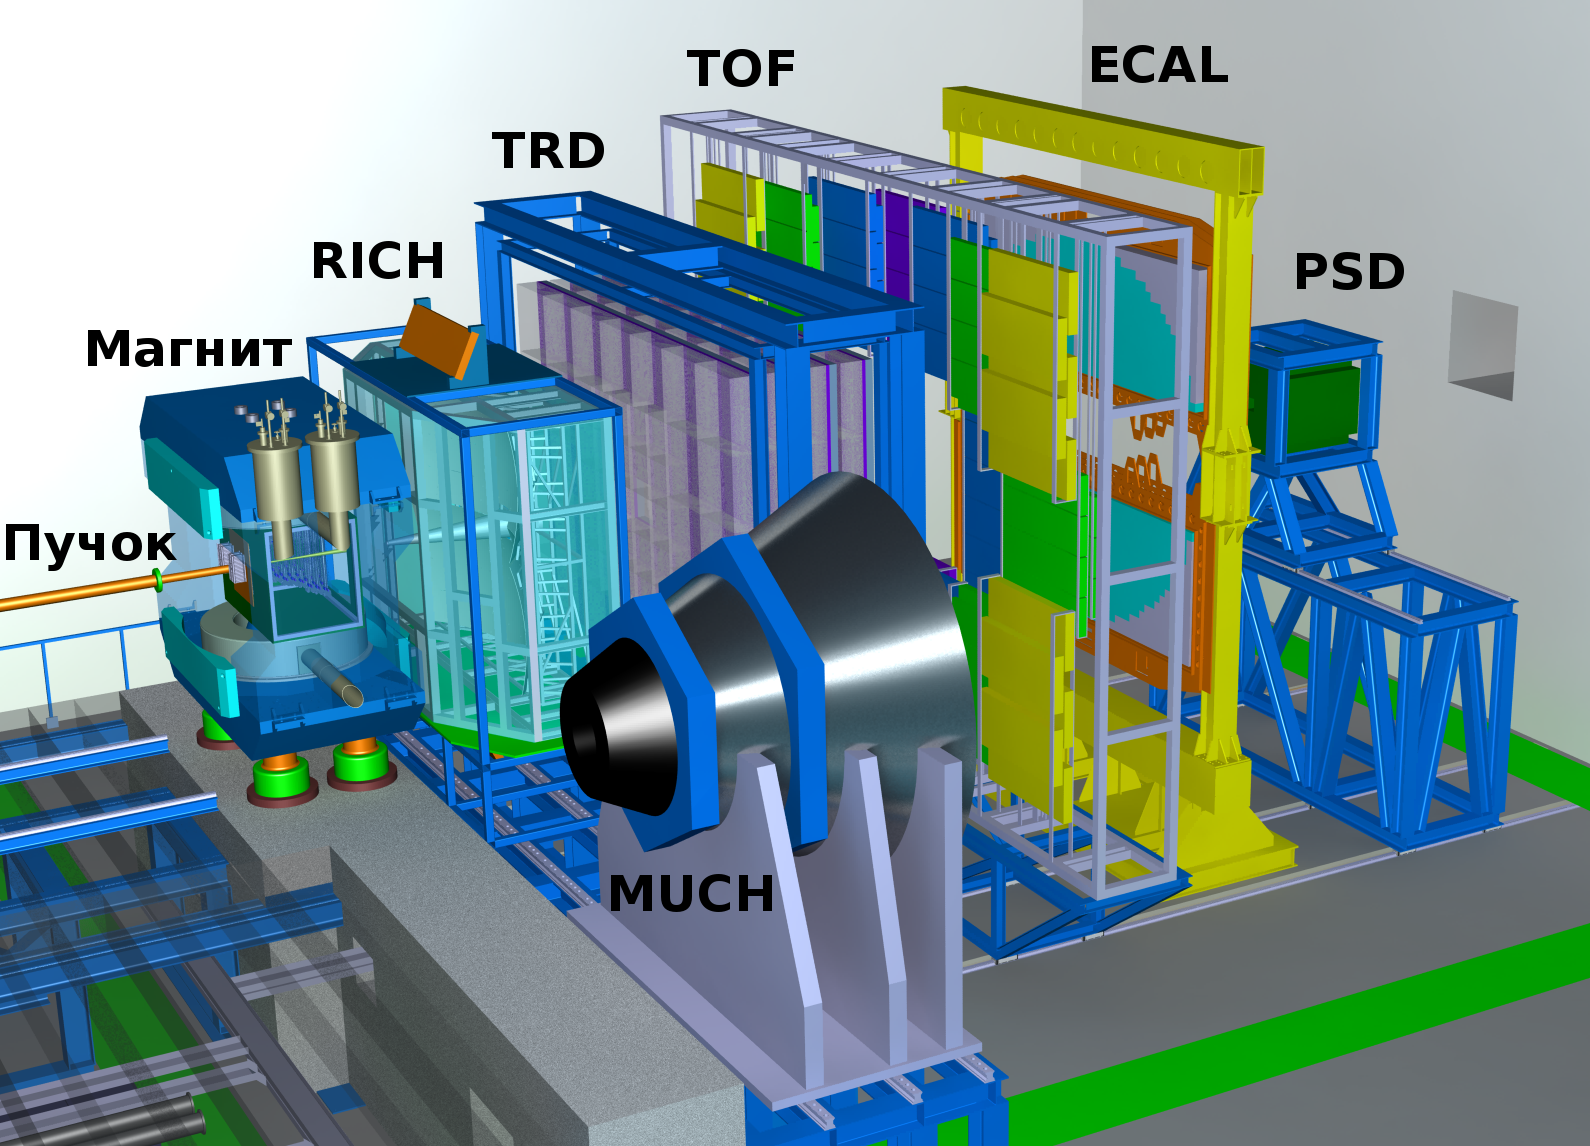
\includegraphics[width=1.0\textwidth]{pictures/1_CBM_SIS100_with_names.png}
\caption{Общий вид экспериментальной установки CBM в конфигурации с RICH.}
\label{fig:CBM}
\end{figure}

Между полюсами сверхпроводящего дипольного магнита~\cite{TDR_Magnet} расположена вакуумная камера, содержащая мишень и вершинный микродетектор (MVD)~\cite{MVD_KOZIEL}, выполненный на основе монолитного пиксельного детектора типа MAPS. Ниже по пучку также между полюсами, но уже вне вакуумной камеры, располагаются станции кремниевой трековой системы (STS)~\cite{TDR_STS}, собранные из двухсторонних микростриповых сенсоров. Координатные трековые детекторы MVD и STS предназначены для реконструкции траекторий заряженных частиц, восстановления их импульсов с точностью не хуже 1\% и нахождения вторичных вершин в условиях высокой множественности и плотности частиц.

Следом за STS в рассматриваемой конфигурации расположен детектор черенковских колец (RICH)~\cite{TDR_RICH}, предназначенный для идентификации электронов и позитронов в диапазоне импульсов от 0.5 ГэВ/с до 8 ГэВ/с с целью восстановления распадов легких векторных мезонов и $ J / \psi $ частиц. Этот детектор, разработке которого посвящена данная статья, имеет радиатор длиной 1.7 м из углекислого газа под небольшим избыточным давлением, систему фокусировки из сегментированных сферических зеркал радиуса 3 м и общей площадью 13 кв.м. В качестве позиционно-чувствительного фотодетектора используется многоанодный фотоэлектронный умножитель Hamamatsu H12700.

Во второй конфигурации на месте RICH стоит мюонная система (MUCH)~\cite{TDR_MUCH}, предназначенная в первую очередь для исследования частиц, распадающихся по димюонному каналу и состоящая из чередующихся слоев железа и газовых трековых камер~\cite{GEM}.

Детектор переходного излучения (TRD) используется для реконструкции треков частиц и идентификации электронов/позитронов в условиях доминирующего фона от пионов~\cite{TRD}.

Для идентификации адронов используется время-пролётный детектор (TOF)~\cite{TDR_TOF}.

Электромагнитный калориметр (ECAL) типа ``шашлык'' необходим для регистрации прямых фотонов и фотонов от распада нейтральных мезонов ($ \pi^{0}, \eta $)~\cite{ECAL_KOROLKO}.

Сегментированный адронный калориметр Projectile Spectator Detector (PSD)~\cite{TDR_PSD} служит для определения центральности столкновения и плоскости реакции путем регистрации ядерных осколков, летящих под малыми углами у пучку.

Эксперимент характеризуется высокой множественностью частиц, большой густотой треков под малыми углами и высокой частотой взаимодействий. Вследствие этого детекторы содержат десятки тысяч плотно упакованных каналов считывания, работающих по бестриггерной схеме, с которых необходимо собирать и анализировать ``на лету'' большой поток данных.

В данной статье описаны результаты тестов прототипа систем регистрации фотонов, считывания, сбора и первичной обработки данных. Были реализованы все принципиальные узлы, как аппаратные, так и программные, соответствующих систем разрабатываемого детектора черенковских колец эксперимента CBM. Тесты проводились как в лабораторных условиях, так и в составе полнофункционального прототипа детектора RICH на пучке PS в ЦЕРН.